\subsection{Цели и методика эксперименального исследования}
Цель экспериментального исследования - проверить эффективность разработаного алгоритма. Для этого алгоритм будет протестирован на нескольких наборах входных данных,  в которых число работ будет варьироваться от 120 до 420, число процессоров - от 4 до 8. Классы графов коррелируют с классами, данными в задаче Хуавей (Приложение 1).

\subsection{Подбор параметоров алгоритма}
Для алгоритма с ограничением сбалансированности нагрузки процессоров были выбраны следующие параметры (для весов, описанных в пункте \ref{sec:get_crit}): $C_1 = 1,\;C_2=0.7$; для алгоритма с ограничением на число межпроцессорных передач - $C_1 = 1,\;C_2 = 0.5,\;C3=0.5$. Заметим, что в дальнейших исследованиях следует переписать алгоритм для работы с допускной системой выбора процессоров для размещения, а так же подбирать параметры не вручную, а при помощи библиотеки \lstinline{hyperopt} \cite{Hyperopt}. Параметр $\Delta = 10$ оставался константным на протяжении всего исследования. Подбор его оптимума - тема для дальнейших исследований.

\subsection{Исследование эффективности алгоритма}

\begin{figure}[H]
    \centering
    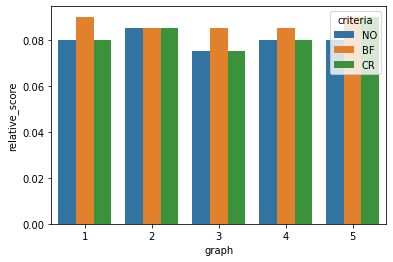
\includegraphics{imgs/relative_score.png}
    \caption{Распределение точности полученного расписания относительно оптимума. Меньше - лучше.}
    \label{pic:relative_score}
\end{figure}

\begin{figure}[H]
    \centering
    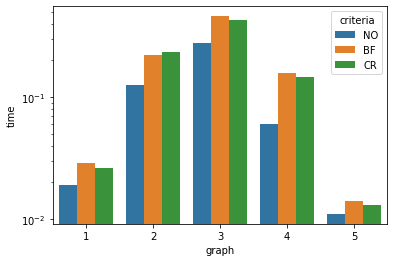
\includegraphics{imgs/times.png}
    \caption{Время выполнения алгоритма на каждом из тестовых графов. Меньше - лучше.}
    \label{pic:times}
\end{figure}

Алгортм бы испытан на пяти наборах входных данных:
\begin{enumerate}
    \item 126 вершин, 4 процессора, 716 передач данных
    \item 417 вершин, 8 процессоров, 2367 передач данных
    \item 408 вершин, 8 процессоров, 8763 передач данных
    \item 396 вершин, 8 процессоров, 395 передачи данных
    \item 93 вершины, 4 процессора, 92 передачи данных
\end{enumerate}

На рисунке \ref{pic:relative_score} представлена относительная точность $score$ алгоритма при расчете на каждом из тестовых графов, расчитанная по формуле:
\begin{equation*}
    score = \frac{\text{время полученного расписания}}{\text{время оптимального расписания}} - 1
\end{equation*}

Дополнительные критерии, упомянутые в \ref{sec:crit}, предствлены на графиках разными цветами.

Из графика видно, что с различными дополнительными критериями алгоритм дает сравнимые времена расписаний. Причина этого - тема для дальнейшего исследования.

На рисунке \ref{pic:times} предоставлено время работы алгоритма для каждого из тестовых графов. Из графа видно, что время работы линейно зависит от количества передач данных между процессорами и количества работ.

В ходе исследования подтвержден факт того, что более $90\%$ работ размещаются в расписании при помощи жадного критерия, упомянутый в \cite{Kostenko_2017}